
\sloppy
\begin{center}{\fontsize{18pt}{18pt}\selectfont Commit Changes \\}\end{center} \par



\begin{figure}[ht]
	\centerline{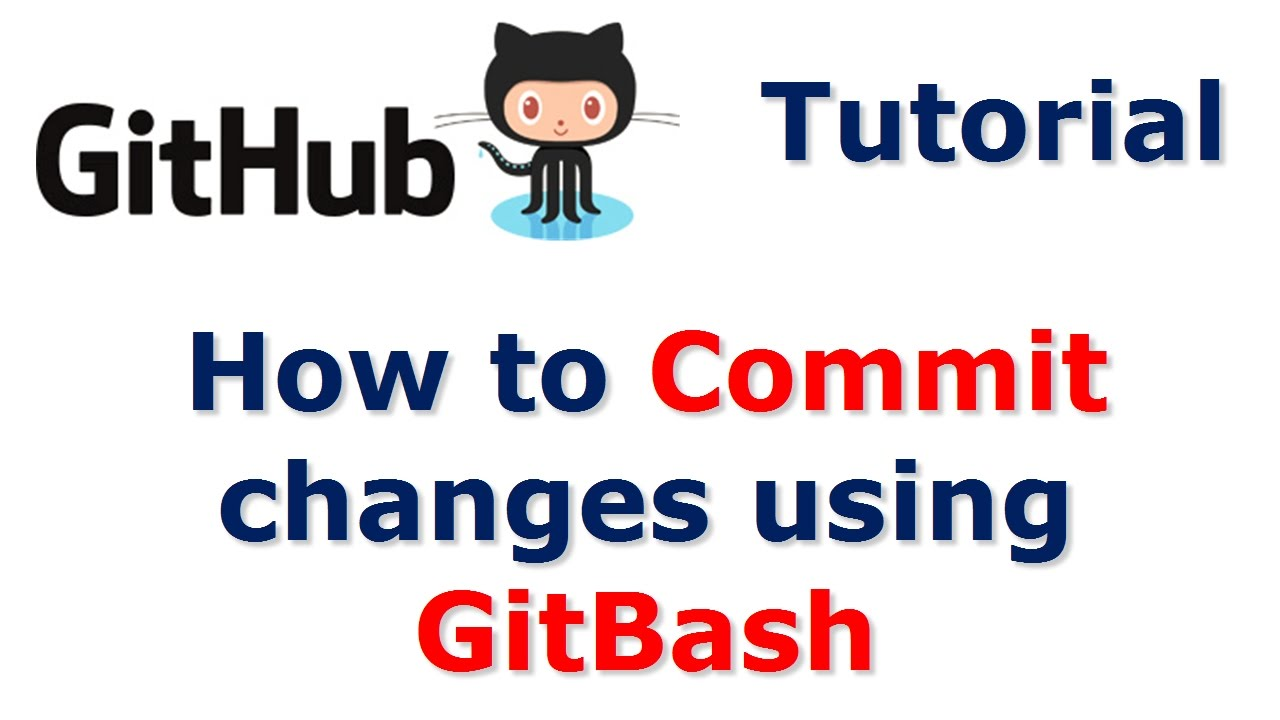
\includegraphics[width=0.80\textwidth]{Figures/dapgit1.jpg}}
	\caption{Commit Changes}
	\label{Commit Changes}
\end{figure}





\section {Pengertian }
\subsection {Commit Changes}


Melakukan perubahan perubahan tentunya anda sudah memiliki repositori Git yang bonafide dan sebuah salinan kerja dari semua berkas untuk proyek tersebut. Anda harus membuat beberapa perubahan dan commit perubahan tersebut ke dalam repositori setiap saat proyek mencapai sebuah keadaan yang ingin Anda rekam.Ingat bahwa setiap berkas di dalam direktori kerja Anda dapat berada di 2 keadaan: terpantau atau tak-terpantau. Berkas terpantau adalah berkas yang sebelumnya berada di snapshot terakhir; mereka dapat berada dalam kondisi belum terubah, terubah, ataupun staged (berada di area stage). Berkas tak-terpantau adalah kebalikannya - merupakan berkas-berkas di dalam direktori kerja yang tidak berada di dalam snapshot terakhir dan juga tidak berada di area staging. Ketika Anda pertama kali menduplikasi sebuah repositori, semua berkas Anda akan terpantau dan belum terubah karena Anda baru saja melakukan checkout dan belum mengubah apapun.Cek Status Anda Alat utama yang Anda gunakan untuk menentukan berkas-berkas mana yang berada dalam keadaan tertentu adalah melalui perintah git status. Jika Anda menggunakan alat ini langsung setelah sebuah clone, Anda akan melihat serupa seperti di bawah ini: \par
\noindent 
 $  \$  $ git status \par
\noindent 
 $  \#  $ On branch master \par
\noindent 
nothing to commit, working directory clean \par
\noindent 
Ini berarti Anda memiliki direktori kerja yang bersih-dengan kata lain, tidak ada berkas terpantau yang terubah. Git juga tidak melihat berkas-berkas yang tak terpantau, karena pasti akan dilaporkan oleh alat ini. Juga, perintah ini memberitahu Anda tentang cabang tempat Anda berada. Pada saat ini, cabang akan selalu berada di master, karena sudah menjadi default-nya; Anda tidak perlu khawatir tentang cabang dulu. Bab berikutnya akan membahas tentang percabangan dan referensi secara lebih detil. \par
\noindent 


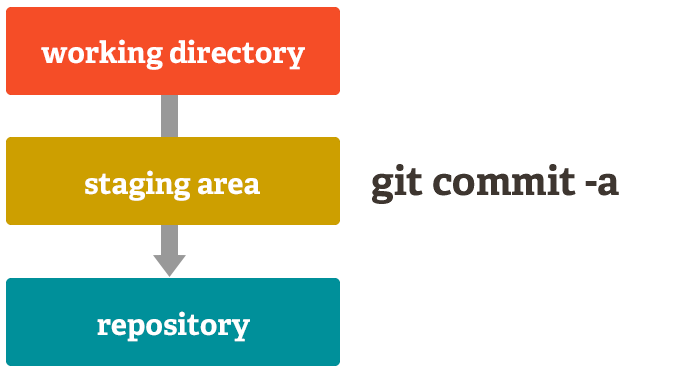
\includegraphics[width=10cm,height=7cm]{Figures/dapigit2.jpg}
\begin{equation}python regular expression\end{equation}





Mari kita umpamakan Anda menambah sebuah berkas baru ke dalam proyek Anda, misalnya sesederhana berkas README. Jika file tersebut belum ada sebelumnya, dan Anda melakukan git status, Anda akan melihatnya sebagai berkas tak-terpantau seperti berikut ini: \par
\vspace{12pt}
\noindent 
\begin{verbatim}
 $  \$  $ vim README \par
\noindent 
 $  \$  $ git status \par
\noindent 
 $  \#  $ On branch master \par
\noindent 
 $  \#  $ Untracked files: \par
\noindent 
 $  \#  $~~ (use "git add <file>..." 
 to include in what will be committed) \par
\noindent 
 $  \#  $ \par
\noindent 
 $  \#  $~~ README \par
\noindent 
nothing added to commit but
 untracked files present (use "git add" to track) 

\end{verbatim}
Anda akan melihat bahwa berkas baru Anda README belum terpantau, karena berada di bawah judul "Untracked files" di keluaran status Anda. Untracked pada dasarnya berarti bahwa Git melihat sebuah berkas yang sebelumnya tidak Anda miliki di snapshot (commit) sebelumnya; Git tidak akan mulai memasukkannya ke dalam snapshot commit hingga Anda secara eksplisit memerintahkan Git. Git berlaku seperti ini agar Anda tidak secara tak-sengaja mulai menyertakan berkas biner hasil kompilasi atau berkas lain yang tidak Anda inginkan untuk disertakan. Anda hanya ingin mulai menyertakan README, mari kita mulai memantau berkas tersebut. \par
\vspace{12pt}
\noindent 
 \section{Berikut adalah langkah-langkah untuk menjalankan perintah}
 
  \begin{enumerate}


\item Untuk mulai memantau berkas baru, Anda menggunakan perintah git add. Untuk mulai memantau berkas README tadi, Anda menjalankannya seperti berikut: \par
\vspace{12pt}
\noindent 
\begin{verbatim}
 $  \$  $ git add README
 
 \end{verbatim}
  \par
\vspace{12pt}
\noindent 

\item Jika Anda menjalankan perintah status lagi, Anda akan melihat bahwa berkas README Anda sekarang sudah terpantau dan sudah masuk ke dalam area stage: \par
\vspace{12pt}
\noindent 

\begin{verbatim}
 $  \$  $ git status \par
\noindent 
 $  \#  $ On branch master \par
\noindent 
 $  \#  $ Changes to be committed: \par
\noindent 
 $  \#  $~~ (use "git reset HEAD <file>..." to unstage) \par
\noindent 
 $  \#  $ \par
\noindent 
 $  \#  $~~~new~file:   README \par
\noindent 
 $  \#  $ \par
\noindent 

 \end{verbatim}

\item Anda dapat mengatakan bahwa berkas tersebut berada di dalam area stage karena tertulis di bawah judul "Changes to be committed". Jika Anda melakukan commit pada saat ini, versi berkas pada saat Anda menjalankan git add inilah yang akan dimasukkan ke dalam sejarah snapshot. Anda mungkin ingat bahwa ketika Anda menjalankan git init sebelumnya, Anda melanjutkannya dengan git add (nama berkas) - yang akan mulai dipantau di direktori Anda. Perintah git add ini mengambil alamat dari berkas ataupun direktori; jika sebuah direktori, perintah tersebut akan menambahkan seluruh berkas yang berada di dalam direktori secara rekursif. \par
\vspace{12pt}
\noindent 

\item Mari kita ubah sebuah berkas yang sudah terpantau. Jika Anda mengubah berkas yang sebelumnya terpantau bernama benchmarks.rb dan kemudian menjalankan perintah status lagi, Anda akan mendapatkan keluaran kurang lebih seperti ini: \par
\vspace{12pt}
\noindent 
\begin{verbatim}
 $  \$  $ git status \par
\noindent 
 $  \#  $ On branch master \par
\noindent 
 $  \#  $ Changes to be committed: \par
\noindent 
 $  \#  $~~ (use "git 
 reset HEAD <file>..." 
 to unstage) \par
\noindent 
 $  \#  $ \par
\noindent 
 $  \#  $~~~new~file:   README \par
\noindent 
 $  \#  $ \par
\noindent 
 $  \#  $ Changes not staged for commit: \par
\noindent 
 $  \#  $~~ (use "git add <file>..."
  to update what will be committed) \par
\noindent 
 $  \#  $ \par
\noindent 
 $  \#  $~~~modified:~  benchmarks.rb \par
\noindent 
 $  \#  $ \par
\vspace{12pt}
\vspace{12pt}
\noindent 
 \end{verbatim}

\item Berkas benchmarks.rb terlihat di bawah bagian yang bernama "Changes not staged for commit" - yang berarti bahwa sebuah berkas terpantau telah berubah di dalam direktori kerja namun belum masuk ke area stage. Untuk memasukkannya ke area stage, Anda menjalankan perintah git add (perintah ini adalah perintah multiguna - Anda menggunakannya untuk mulai memantau berkas baru, untuk memasukkannya ke area stage, dan untuk melakukan hal lain seperti menandai berkas terkonflik menjadi terpecahkan). Mari kita sekarang jalankan git add untuk memasukkan berkas benchmarks.rb ke dalam area stage, dan jalankan git status lagi: \par
\vspace{12pt}
\noindent 

\begin{verbatim}


 $  \$  $ git add benchmarks.rb \par
\noindent 
 $  \$  $ git status \par
\noindent 
 $  \#  $ On branch master \par
\noindent 
 $  \#  $ Changes to be committed: \par
\noindent 
 $  \#  $~~ (use "git reset HEAD
  <file>..." to unstage) \par
\noindent 
 $  \#  $ \par
\noindent 
 $  \#  $~~~new~file:   README \par
\noindent 
 $  \#  $~~~modified:~  benchmarks.rb \par
\noindent 
 $  \#  $ \par
\vspace{12pt}
\vspace{12pt}
\vspace{12pt}
\noindent 

\end{verbatim}

\item Kedua file sekarang berada di area stage dan akan masuk ke dalam commit Anda berikutnya. Pada saat ini, semisal Anda teringat satu perubahan yang Anda ingin buat di benchmarks.rb sebelum Anda lakukan commit. Anda buka berkas tersebut kembali dan melakukan perubahan tersebut, dan Anda siap untuk melakukan commit. Namun, mari kita coba jalankan git status kembali: \par
\vspace{12pt}
\vspace{12pt}
\vspace{12pt}
\noindent 

\begin{verbatim}



 $  \$  $ vim benchmarks.rb  \par
\noindent 
 $  \$  $ git status \par
\noindent 
 $  \#  $ On branch master \par
\noindent 
 $  \#  $ Changes to be committed: \par
\noindent 
 $  \#  $~~ (use "git reset HEAD <file>..."
  to unstage) \par
\noindent 
 $  \#  $ \par
\noindent 
 $  \#  $~~~new~file:   README \par
\noindent 
 $  \#  $~~~modified:~  benchmarks.rb \par
\noindent 
 $  \#  $ \par
\noindent 
 $  \#  $ Changes not staged for commit: \par
\noindent 
 $  \#  $~~ (use "git add <file>..."
  to update what will be committed) \par
\noindent 
 $  \#  $ \par
\noindent 
 $  \#  $~~~modified:~  benchmarks.rb \par
\noindent 
 $  \#  $ \par
\vspace{12pt}
\noindent 
\end{verbatim}


\item Apa? Sekarang benchmarks.rb terdaftar di dua tempat: area stage dan area terubah. Bagaimana hal ini bisa terjadi? Ternyata Git memasukkan berkas ke area stage tepat seperti ketika Anda menjalankan perintah git add. Jika Anda commit sekarang, versi benchmarks.rb pada saat Anda terakhir lakukan perintah git add-lah yang akan masuk ke dalam commit, bukan versi berkas yang saat ini terlihat di direktori kerja Anda ketika Anda menjalankan git commit. Jika Anda mengubah sebuah berkas setelah Anda menjalankan git add, Anda harus menjalankan git add kembali untuk memasukkan versi berkas terakhir ke dalam area stage: \par
\vspace{12pt}
\vspace{12pt}
\noindent 

\begin{verbatim}



 $  \$  $ git add benchmarks.rb \par
\noindent 
 $  \$  $ git status \par
\noindent 
 $  \#  $ On branch master \par
\noindent 
 $  \#  $ Changes to be committed: \par
\noindent 
 $  \#  $~~ (use "git reset HEAD <file>..."
  to unstage) \par
\noindent 
 $  \#  $ \par
\noindent 
 $  \#  $~~~new~file:   README \par
\noindent 
 $  \#  $~~~modified:~  benchmarks.rb \par
\noindent 
 $  \#  $ \par
 
 \end{verbatim}
 
\vspace{12pt}
\vspace{12pt}
\noindent 


\end{enumerate}

\section{Tambahkan secara otomatis}

Terkadang, Anda memiliki sekumpulan berkas yang Anda tidak ingin Git tambahkan secara otomatis atau bahkan terlihat sebagai tak-terpantau. Biasanya berkas hasil keluaran seperti berkas log atau berkas yang dihasilkan oleh sistem build Anda. Dalam kasus ini, Anda dapat membuat sebuah berkas bernama .gitignore yang berisi pola dari berkas terabaikan. Berikut adalah sebuah contoh isi dari berkas .gitignore: \par
\noindent 
 $  \$  $ cat .gitignore \par
\noindent 
*.[oa] \par
\noindent 
* $  \sim  $ \par
\noindent 
Baris pertama memberitahu Git untuk mengabaikan semua file yang berakhiran .o atau .a - berkas object dan arsip yang mungkin dihasilkan dari kompilasi kode Anda. Baris kedua memberitahu Git untuk mengabaikan semua file yang berakhiran dengan sebuah tilde ( $  \sim  $), yang biasanya digunakan oleh banyak aplikasi olah-kata seperti Emacs untuk menandai berkas sementara. Anda juga dapat memasukkan direktori log, tmp ataupun pid; dokumentasi otomatis; dan lainnya. Menata berkas .gitignore sebelum Anda mulai bekerja secara umum merupakan ide yang baik sehingga Anda tidak secara tak-sengaja melakukan commit terhadap berkas yang sangat tidak Anda inginkan berada di dalam repositori Git. \par
\noindent 
Aturan untuk pola yang dapat Anda gunakan di dalam berkas .gitignore adalah sebagai berikut: \par
\noindent 
\begin{itemize}
\item Baris kosong atau baris dimulai dengan  $  \#  $ akan diabaikan. \par
\noindent 
\item Pola glob standar dapat digunakan. \par
\noindent 
\item Anda dapat mengakhir pola dengan sebuah slash (/) untuk menandai sebuah direktori. \par
\noindent 
\item Anda dapat menegasikan sebuah pola dengan memulainya menggunakan karakter tanda seru (!).\end{itemize}
 \par
\noindent 
Pola Glob adalah seperti regular expression yang disederhanakan yang biasanya digunakan di shell. Sebuah asterisk (*) berarti 0 atau lebih karakter; [abc] terpasangkan dengan karakter apapun yang ditulis dalam kurung siku (dalam hal ini a, b, atau c); sebuah tanda tanya (?) terpasangkan dengan sebuah karakter; dan kurung siku yang melingkupi karakter yang terpisahkan dengan sebuah tanda hubung([0-9]) terpasangkan dengan karakter apapun yang berada diantaranya (dalam hal ini 0 hingga 9). \par
\noindent 
Berikut adalah contoh lain dari isi berkas .gitignore: \par
\noindent 
 $  \#  $ sebuah komentar – akan diabaikan \par
\noindent 
 $  \#  $ abaikan berkas .a \par
\noindent 
*.a \par
\noindent 
 $  \#  $ tapi pantau lib.a, walaupun Anda abaikan berkas .a di atas \par
\noindent 
!lib.a \par
\noindent 
 $  \#  $ hanya abaikan berkas TODO yang berada di rooto, bukan di subdir/TODO \par
\noindent 
/TODO \par
\noindent 
 $  \#  $ abaikan semua berkas di dalam direktori build/ \par
\noindent 
build/ \par
\noindent 
 $  \#  $ abaikan doc/notes.txt, tapi bukan doc/server/arch.txt \par
\noindent 
doc/*.txt \par
\noindent 
Jika perintah git status terlalu kabur untuk Anda - Anda ingin mengetahui secara pasti apa yang telah berubah, bukan hanya berkas mana yang berubah - Anda dapat menggunakan perintah git diff. Kita akan bahas git diff secara lebih detil nanti; namun Anda mungkin menggunakannya paling sering untuk menjawab 2 pertanyaan berikut: Apa yang Anda ubah tapi belum dimasukkan ke area stage? Dan apa yang telah Anda ubah yang akan segera Anda commit? Walaupun git status menjawab pertanyaan tersebut secara umum, git diff menunjukkan kepada Anda dengan tepat baris yang ditambahkan dan dibuang - dalam bentuk patch-nya. \par
\noindent 
Mari kita anggap Anda mengubah dan memasukkan berkas README ke area stage lagi dan kemudian mengubah berkas benchmarks.rb tanpa memasukkannya ke area stage. Jika Anda jalankan perintah status Anda, Anda akan sekali lagi melihat keluaran seperti berikut: \par
\vspace{12pt}
\noindent 
git status \par
\noindent 
 $  \#  $ On branch master \par
\noindent 
 $  \#  $ Changes to be committed: \par
\noindent 
 $  \#  $~~ (use "git reset HEAD <file>..." to unstage) \par
\noindent 
 $  \#  $ \par
\noindent 
 $  \#  $~~~new~file:   README \par
\noindent 
 $  \#  $ \par
\noindent 
 $  \#  $ Changes not staged for commit: \par
\noindent 
 $  \#  $~~ (use "git add <file>..." to update what will be committed) \par
\noindent 
 $  \#  $ \par
\noindent 
 $  \#  $~~~modified:~  benchmarks.rb \par
\noindent 
 $  \#  $ \par
\noindent 
Untuk melihat apa yang Anda telah ubah namun belum masuk ke area stage, ketikkan git diff tanpa argumen lainnya. \par
\vspace{12pt}
\noindent 
git diff \par
\noindent 
diff --git a/benchmarks.rb b/benchmarks.rb \par
\noindent 
index 3cb747f..da65585 100644 \par
\noindent 
--- a/benchmarks.rb \par
\noindent 
+++ b/benchmarks.rb \par
\noindent 
@@ -36,6 +36,10 @@ def main \par
\noindent 
~~~~~~~~~~ @commit.parents[0].parents[0].parents[0] \par
\noindent 
~~~~~~~~ end \par
\vspace{12pt}
\noindent 
+~~~~~~~ run $  \_  $code(x, 'commits 1') do \par
\noindent 
+~~~~~~~~~ git.commits.size \par
\noindent 
+~~~~~~~ end \par
\noindent 
+ \par
\noindent 
~~~~~~~~ run $  \_  $code(x, 'commits 2') do \par
\noindent 
~~~~~~~~~~ log = git.commits('master', 15) \par
\noindent 
~~~~~~~~~~ log.size \par
\noindent 
Perintah di atas membandingkan apa yang ada di direktori kerja Anda dengan apa yang ada di area stage. Hasilnya memberitahu Anda bahwa perubahan yang Anda ubah namun belum masuk ke area stage. \par
\noindent 
Jika Anda ingin melihat apa yang telah Anda masukkan ke area stage yang nantinya akan masuk ke commit Anda berikutnya, Anda dapat menggunakan git diff --cached. (Di Git versi 1.6.1 atau yang lebih tinggi, Anda dapat juga menggunakan git diff --staged, yang mungkin lebih mudah untuk diingat). Perintah ini membandingkan area stage Anda dengan commit Anda terakhir: \par
\vspace{12pt}
\vspace{12pt}
\noindent 
 $  \$  $ git diff --cached \par
\noindent 
diff --git a/README b/README \par
\noindent 
new file mode 100644 \par
\noindent 
index 0000000..03902a1 \par
\noindent 
--- /dev/null \par
\noindent 
+++ b/README2 \par
\noindent 
@@ -0,0 +1,5 @@ \par
\noindent 
+grit \par
\noindent 
+ by Tom Preston-Werner, Chris Wanstrath \par
\noindent 
+ http://github.com/mojombo/grit \par
\noindent 
+ \par
\noindent 
+Grit is a Ruby library for extracting information from a Git repository \par
\noindent 
Satu hal penting yang harus dicatat adalah bahwa git diff saja tidak memperlihatkan semua perubahan yang telah Anda lakukan sejak terakhir Anda commit - hanya perubahan yang belum masuk ke area stage saja. Mungkin agak sedikit membingungkan, karena jika Anda telah memasukkan semua perubahan ke area stage, git diff akan memberikan keluaran kosong. \par
\noindent 
Sebagai contoh lain, jika Anda memasukkan berkas benchmarks.rb ke area stage dan kemudian meng-editnya, Anda dapat menggunakan git diff untuk melihat perubahan di berkas tersebut yang telah masuk ke area stage dan perubahan yang masih di luar area stage: \par
\noindent 
 $  \$  $ git add benchmarks.rb \par
\noindent 
 $  \$  $ echo ' $  \#  $ test line' >> benchmarks.rb \par
\noindent 
 $  \$  $ git status \par
\noindent 
 $  \#  $ On branch master \par
\noindent 
 $  \#  $ \par
\noindent 
 $  \#  $ Changes to be committed: \par
\noindent 
 $  \#  $ \par
\noindent 
 $  \#  $~~~modified:~  benchmarks.rb \par
\noindent 
 $  \#  $ \par
\noindent 
 $  \#  $ Changes not staged for commit: \par
\noindent 
 $  \#  $ \par
\noindent 
 $  \#  $~~~modified:~  benchmarks.rb \par
\noindent 
 $  \#  $ \par
\noindent 
Sekarang Anda dapat menggunakan git diff untuk melihat apa saja yang masih belum dimasukkan ke area stage: \par
\vspace{12pt}
\noindent 
 $  \$  $ git diff  \par
\noindent 
diff --git a/benchmarks.rb b/benchmarks.rb \par
\noindent 
index e445e28..86b2f7c 100644 \par
\noindent 
--- a/benchmarks.rb \par
\noindent 
+++ b/benchmarks.rb \par
\noindent 
@@ -127,3 +127,4 @@ end \par
\noindent 
 main() \par
\vspace{12pt}
\noindent 
  $  \#  $ $  \#  $pp Grit::GitRuby.cache $  \_  $client.stats  \par
\noindent 
+ $  \#  $ test line \par
\vspace{12pt}
\noindent 
dan git diff --cached untuk melihat apa yang telah Anda masukkan ke area stage sejauh ini: \par
\vspace{12pt}
\noindent 
 $  \$  $ git diff --cached \par
\noindent 
diff --git a/benchmarks.rb b/benchmarks.rb \par
\noindent 
index 3cb747f..e445e28 100644 \par
\noindent 
--- a/benchmarks.rb \par
\noindent 
+++ b/benchmarks.rb \par
\noindent 
@@ -36,6 +36,10 @@ def main \par
\noindent 
~~~~~~~~~ @commit.parents[0].parents[0].parents[0] \par
\noindent 
~~~~~~~ end \par
\vspace{12pt}
\noindent 
+~~~~~~~ run $  \_  $code(x, 'commits 1') do \par
\noindent 
+~~~~~~~~~ git.commits.size \par
\noindent 
+~~~~~~~ end \par
\noindent 
+~~~~~~~~~~~~~  \par
\noindent 
~~~~~~~ run $  \_  $code(x, 'commits 2') do \par
\noindent 
~~~~~~~~~ log = git.commits('master', 15) \par
\noindent 
~~~~~~~~~ log.size \par
\vspace{12pt}
\vspace{12pt}
\noindent 
Sekarang setelah area stage Anda tertata sebagaimana yang Anda inginkan, Anda dapat melakukan commit terhadap perubahan Anda. Ingat bahwa apapun yang masih di luar area stage - berkas apapun yang Anda telah buat atau ubah yang belum Anda jalankan git add terhadapnya sejak terakhir Anda edit - tidak akan masuk ke dalam commit ini. Perubahan tersebut akan tetap sebagai berkas terubah di cakram Anda. Dalam hal ini, saat terakhir Anda jalankan git status, Anda telah melihat bahwa semuanya telah masuk ke stage, sehingga Anda siap untuk melakukan commit dari perubahan Anda. Cara termudah untuk melakukan commit adalah dengan mengetikkan git commit: \par
\vspace{12pt}
\noindent 
 $  \$  $ git commit \par
\noindent 
Dengan melakukan ini, aplikasi olahkata pilihan Anda akan terjalankan (Ini ditata oleh variabel lingkungan  $  \$  $EDITOR di shell Anda - biasanya vim atau emacs, walaupun Anda dapat mengkonfigurasinya dengan apapun yang Anda inginkan menggunakan perintah git config -- global core.editor yang telah Anda lihat di Bab 1). \par
\noindent 
Aplikasi olahkata akan menampilakn teks berikut (contoh berikut adalah dari layar Vim): \par
\vspace{12pt}
\vspace{12pt}
\noindent 
 $  \#  $ Please enter the commit message for your changes. Lines starting \par
\noindent 
 $  \#  $ with ' $  \#  $' will be ignored, and an empty message aborts the commit. \par
\noindent 
 $  \#  $ On branch master \par
\noindent 
 $  \#  $ Changes to be committed: \par
\noindent 
 $  \#  $~~ (use "git reset HEAD <file>..." to unstage) \par
\noindent 
 $  \#  $ \par
\noindent 
 $  \#  $~~~~~~~new~file:   README \par
\noindent 
 $  \#  $~~~~~~~modified:~  benchmarks.rb  \par
\noindent 
 $  \sim  $ \par
\noindent 
 $  \sim  $ \par
\noindent 
 $  \sim  $ \par
\noindent 
".git/COMMIT $  \_  $EDITMSG" 10L, 283C \par
\vspace{12pt}
\vspace{12pt}
\noindent 
Anda dapat melihat bahwa pesan commit standar berisi keluaran terakhir dari perintah git status yang terkomentari dan sebuah baris kosong di bagian atas. Anda dapat membuang komentar-komentar ini dan mengetikkan pesan commit Anda, atau Anda dapat membiarkannya untuk membantu Anda mengingat apa yang akan Anda commit. (Untuk pengingat yang lebih eksplisit dari apa yang Anda ubah, Anda dapat menggunakan opsi -v di perintah git commit. Melakukan hal ini akan membuat diff dari perubahan Anda di dalam olahkata sehingga Anda dapat melihat secara tepat apa yang telah Anda lakukan). Ketika Anda keluar dari olahkata, Git akan membuat commit Anda dengan pesan yang Anda buat (dengan bagian terkomentari dibuang). \par
\noindent 
Cara lainnya, Anda dapat mengetikkan pesan commit Anda sebaris denegan perintah commit dengan mencantumkannya setelah tanda -m seperti berikut: \par
\vspace{12pt}
\vspace{12pt}
\noindent 
 $  \$  $ git commit -m "Story 182: Fix benchmarks for speed" \par
\noindent 
[master]: created 463dc4f: "Fix benchmarks for speed" \par
\noindent 
 2 files changed, 3 insertions(+), 0 deletions(-) \par
\noindent 
 create mode 100644 README \par
\vspace{12pt}
\vspace{12pt}
\noindent 
Sekarang Anda telah membuat commit pertama Anda $  \sim  $ Anda dapat lihat bahwa commit tersebut telah memberi Anda beberapa keluaran tentang dirinya sendiri: cabang apa yang Anda jadikan target commit (master), ceksum SHA-1 apa yang commit tersebut miliki (463dc4f), berapa banyak berkas yang diubah, dan statistik tentang jumlah baris yang ditambah dan dibuang dalam commit tersebut. \par
\noindent 
Ingat bahwa commit merekam snapshot yang Anda telah tata di area stage. Apapun yang tidak Anda masukkan ke area stage akan tetap berada di tempatnya, tetap dalam keadaan terubah; Anda dapat melakukan commit lagi untuk memasukkannya ke dalam sejarah Anda. Setiap saat Anda melakukan sebuah commit, Anda merekamkan sebuah snapshot dari proyek Anda yang bisa Anda kembalikan atau Anda bandingkan nantinya. \par
\noindent 
Walaupun dapat menjadi sangat berguna untuk menata commit tepat sebagaimana Anda inginkan, area stage terkadang sedikit lebih kompleks dibandingkan apa yang Anda butuhkan di dalam alurkerja Anda. Jika Anda ingin melewatkan area stage, Git menyediakan sebuah jalan pintas sederhana. Dengan memberikan opsi -a ke perintah git commit akan membuat Git secara otomatis menempatkan setiap berkas yang telah terpantau ke area stage sebelum melakukan commit, membuat Anda dapat melewatkan bagian git add: \par
\vspace{12pt}
\noindent 
 $  \$  $ git status \par
\noindent 
 $  \#  $ On branch master \par
\noindent 
 $  \#  $ \par
\noindent 
 $  \#  $ Changes not staged for commit: \par
\noindent 
 $  \#  $ \par
\noindent 
 $  \#  $~~~modified:~  benchmarks.rb \par
\noindent 
 $  \#  $ \par
\noindent 
 $  \$  $ git commit -a -m 'added new benchmarks' \par
\noindent 
[master 83e38c7] added new benchmarks \par
\noindent 
 1 files changed, 5 insertions(+), 0 deletions(-) \par
\vspace{12pt}
\noindent 
Perhatikan bagaimana Anda tidak perlu menjalankan git add terhadap berkas benchmarks.rb dalam hal ini sebelum Anda commit. \par
\noindent 
\textbf{M}\textbf{enghapus sebuah berkas dari Git} \par
\noindent 
Untuk menghapus sebuah berkas dari Git, Anda harus menghapusnya dari berkas terpantau (lebih tepatnya, mengpus dari area stage) dan kemudian commit. Perintah git rm melakukan hal tadi dan juga menghapus berkas tersebut dari direktori kerja Anda sehingga Anda tidak melihatnya sebagai berkas yang tak terpantau nantinya. \par
\noindent 
Jika Anda hanya menghapus berkas dari direktori kerja Anda, berkas tersebut akan muncul di bagian "Changes not staged for commit" (yaitu, di luar area stage) dari keluaran git status Anda: \par
\noindent 
 $  \$  $ rm grit.gemspec \par
\noindent 
 $  \$  $ git status \par
\noindent 
 $  \#  $ On branch master \par
\noindent 
 $  \#  $ \par
\noindent 
 $  \#  $ Changes not staged for commit: \par
\noindent 
 $  \#  $~~ (use "git add/rm <file>..." to update what will be committed) \par
\noindent 
 $  \#  $ \par
\noindent 
 $  \#  $~~~~~~~deleted:~~  grit.gemspec \par
\noindent 
 $  \#  $ \par
\vspace{12pt}
\vspace{12pt}
\noindent 
Kemudian, jika Anda jalankan git rm, Git akan memasukkan penghapusan berkas tersebut ke area stage: \par
\vspace{12pt}
\noindent 
 $  \$  $ git rm grit.gemspec \par
\noindent 
rm 'grit.gemspec' \par
\noindent 
 $  \$  $ git status \par
\noindent 
 $  \#  $ On branch master \par
\noindent 
 $  \#  $ \par
\noindent 
 $  \#  $ Changes to be committed: \par
\noindent 
 $  \#  $~~ (use "git reset HEAD <file>..." to unstage) \par
\noindent 
 $  \#  $ \par
\noindent 
 $  \#  $~~~~~~~deleted:~~  grit.gemspec \par
\noindent 
 $  \#  $ \par
\vspace{12pt}
\vspace{12pt}
\noindent 
Pada saat Anda commit nantinya, berkas tersebut akan hilang dan tidak lagi terpantau. Jika Anda mengubah berkas tersebut dan menambahkannya lagi ke index, Anda harus memaksa penghapusannya dengan menggunakan opsi -f. Ini adalah fitur keamanan (safety) untuk mencegah ketidaksengajaan penghapusan terhadap data yang belum terekam di dalam snapshot dan tak dapat dikembalikan oleh Git. \par
\noindent 
Hal berguna lain yang Anda dapat lakukan adalah untuk tetap menyimpan berkas di direktori kerja tetapi menghapusnya dari area kerja. Dengan kata lain, Anda mungkin ingin tetap menyimpan berkas tersebut di dalam cakram keras tetapi tidak ingin Git untuk memantaunya lagi. Hal ini khususnya berguna jika Anda lupa untuk menambahkan sesuaitu ke berkas .gitignore Anda dan secara tak-sengaja menambahkannya, seperti sebuah berkas log yang besar, atau sekumpulan berkas hasil kompilasi .a. Untuk melakukan ini, gunakan opsi --cached: \par
\vspace{12pt}
\noindent 
 $  \$  $ git rm --cached readme.txt \par
\noindent 
Anda dapat menambahkan nama berkas, direktori, dan pola glob ke perintah git rm. Ini berarti Anda dapat melakukan hal seperti \par
\vspace{12pt}
\noindent 
 $  \$  $ git rm log/ $  \setminus  $*.log \par
\noindent 
Perhatikan karakter backslash ( $  \setminus  $) di depan tanda *. Ini dibutuhkan agar Git juga meng-ekspansi nama berkas sebagai tambahan dari ekspansi nama berkas oleh shell Anda. Perintah ini mengapus semua berkas yang memiliki ekstensi .log di dalam direktori log/. Atau, Anda dapat melakukannya seperti ini: \par
\noindent 
 $  \$  $ git rm  $  \setminus  $* $  \sim  $ \par
\noindent 
Tidak seperti kebanyakan sistem VCS lainnya, Git tidak secara eksplisit memantau perpindahan berkas. Jika Anda mengubag nama berkas di Git, tidak ada metada yang tersimpan di Git yang menyatakan bahwa Anda mengubah nama berkas tersebut. Namun demikian, Git cukup cerdas untuk menemukannya berdasarkan fakta yang ada - kita akan membicarakan tentang mendeteksi perpindahan berkas sebentar lagi. \par
\noindent 
Untuk itu agak membingungkan bahwa Git memiliki perintah mv. Jika Anda hendak mengubah nama berkas di Git, Anda dapat menjalankan seperti berikut \par
\noindent 
 $  \$  $ git mv file $  \_  $from file $  \_  $to \par
\noindent 
dan itu berjalan baik. Bahkan, jika Anda menjalankannya seperti ini kemudian melihat ke status, Anda akan melihat bahwa Git menganggapnya sebagai perintah pengubahan nama berkas.  \par
\noindent 
 $  \$  $ git mv README.txt README \par
\noindent 
 $  \$  $ git status \par
\noindent 
 $  \#  $ On branch master \par
\noindent 
 $  \#  $ Your branch is ahead of 'origin/master' by 1 commit. \par
\noindent 
 $  \#  $ \par
\noindent 
 $  \#  $ Changes to be committed: \par
\noindent 
 $  \#  $~~ (use "git reset HEAD <file>..." to unstage) \par
\noindent 
 $  \#  $ \par
\noindent 
 $  \#  $~~~~~~~renamed:~~  README.txt -> README \par
\noindent 
 $  \#  $ \par
\noindent 
Namun sebetulnya hal ini serupa dengan menjalankan perintah-perintah berikut: \par
\noindent 
 $  \$  $ mv README.txt README \par
\noindent 
 $  \$  $ git rm README.txt \par
\noindent 
 $  \$  $ git add README \par
\noindent 
Git mengetahui secara implisit bahwa perubahan yang terjadi merupakan proses pengubahan nama, sehingga sebetulnya tidaklah terlalu bermasalah jika Anda mengubah nama sebuah berkas dengan cara ini atau dengan menggunakan perintah mv. Satu-satunya perbedaan utama adalah mv berjumlah satu perintah dan bukannya tiga - yang membuat fungsi ini lebih nyaman digunakan. Lebih penting lagi, Anda sebetulnya dapat menggunakan alat apapun yang Anda suka untuk mengubah nama berkas, tinggal tambahkan perintah add/rm di bagian akhir, sesaat sebelum Anda melakukan commit. \par
\vspace{12pt}
\vspace{12pt}
\vspace{12pt}
\vspace{12pt}
